% Diapo des avancements

\begin{frame}[c]
  \frametitle{Avancement sur la qualité du réseau en PH et de la compréhension des paramètres}
  
 \begin{center}
  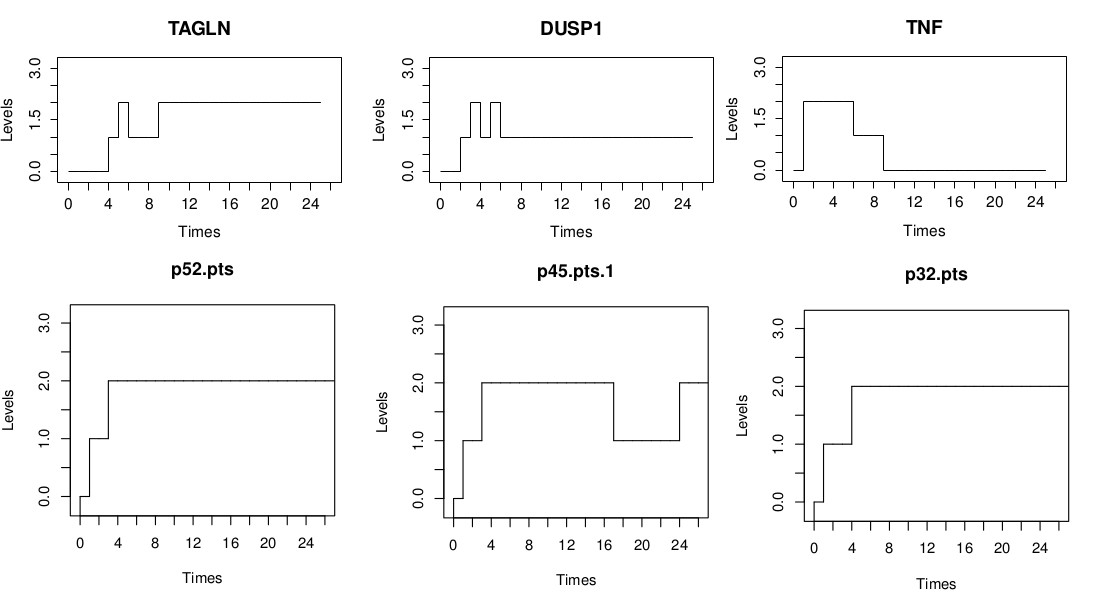
\includegraphics[scale=0.2]{figs/ph10-5-1.jpg}
\end{center}


\pause
\begin{itemize}
  \item Le temps de propagation du signal dans le réseau.
  \item Les simulations pour $r_{a}= r_{i}=10.0$ et $sa = 50 $
\end{itemize}

\textcolor{couleurtheme}{$\Rightarrow$} \fbox{\tval{\large Analyse???}} \textcolor{couleurtheme}{$\Leftarrow$}

\end{frame}

\begin{frame}[c]
  \frametitle{Avancement sur la qualité du réseau en PH et de la compréhension des paramètres}
  
 \begin{center}
  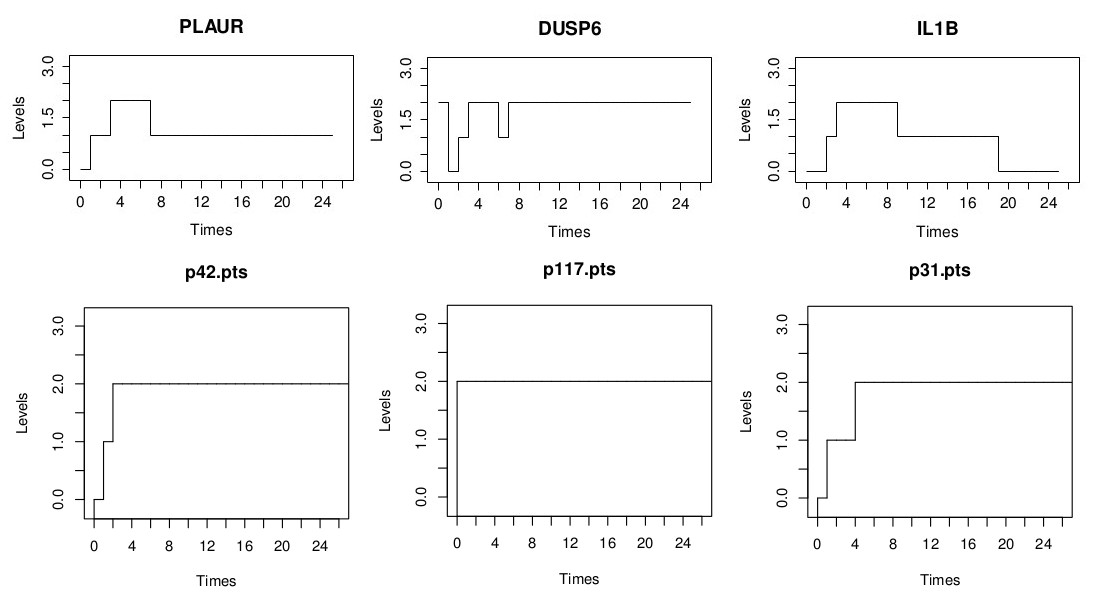
\includegraphics[scale=0.2]{figs/ph10-5-2.jpg}
\end{center}


\pause
\begin{itemize}
  \item Le temps de propagation du signal dans le réseau.
  \item Les simulations pour $r_{a}= r_{i}=10.0$ et $sa = 50 $
\end{itemize}

\textcolor{couleurtheme}{$\Rightarrow$} \fbox{\tval{\large Analyse???}} \textcolor{couleurtheme}{$\Leftarrow$}

\end{frame}

\begin{frame}[c]
  \frametitle{Avancement sur la qualité du réseau en PH et de la compréhension des paramètres}
  
 \begin{center}
  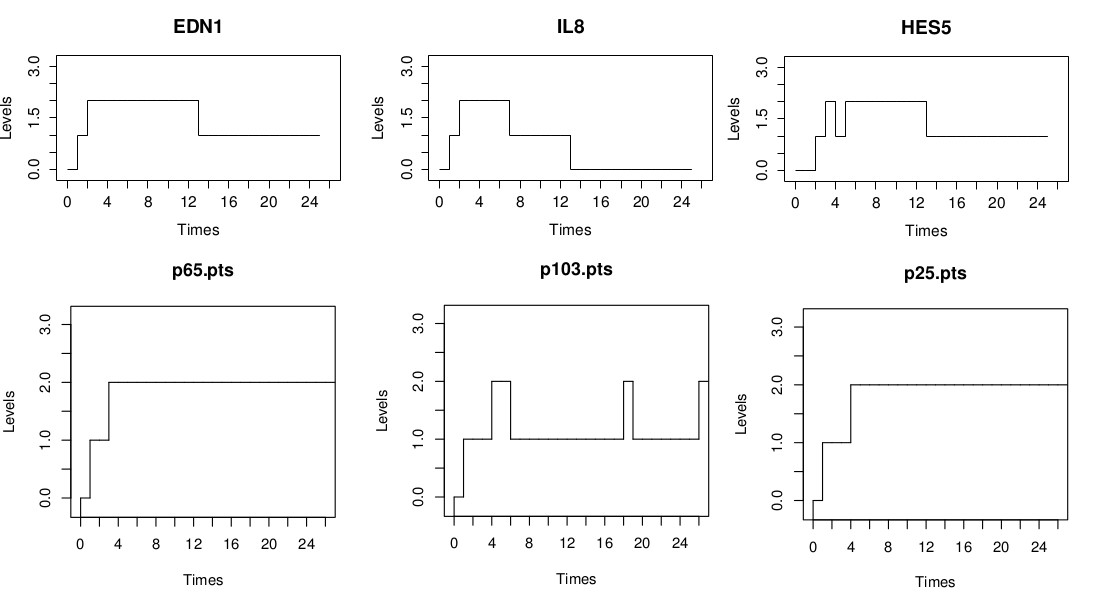
\includegraphics[scale=0.2]{figs/ph10-5-3.jpg}
\end{center}


\pause
\begin{itemize}
  \item Le temps de propagation du signal dans le réseau.
  \item Les simulations pour $r_{a}= r_{i}=10.0$ et $sa = 50 $
\end{itemize}

\textcolor{couleurtheme}{$\Rightarrow$} \fbox{\tval{\large Analyse???}} \textcolor{couleurtheme}{$\Leftarrow$}

\end{frame}

\begin{frame}[c]
  \frametitle{Avancement sur la qualité du réseau en PH et de la compréhension des paramètres}
  
 \begin{center}
  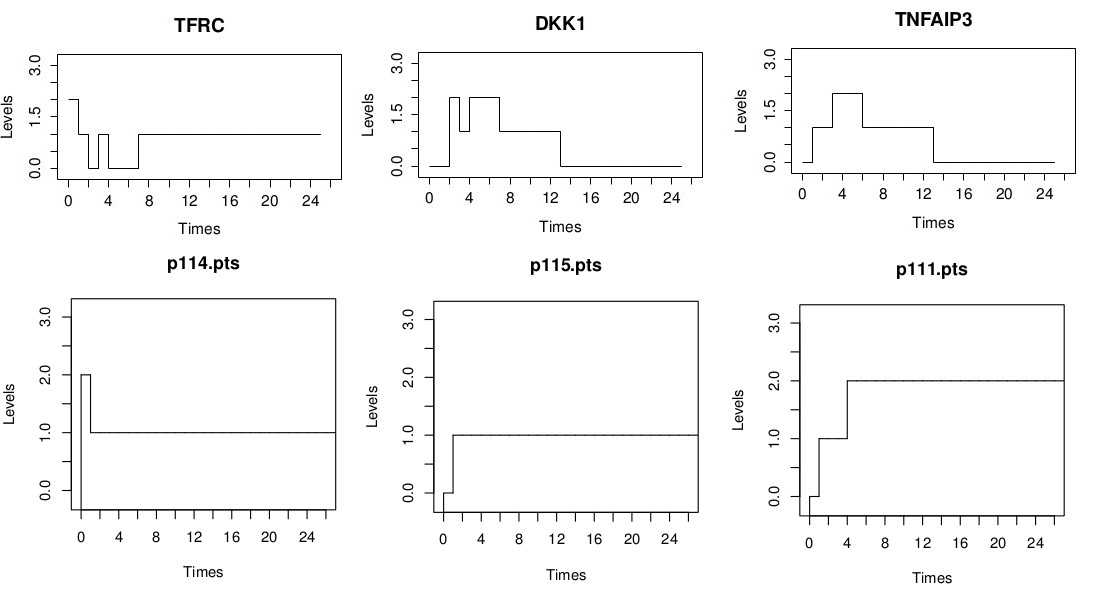
\includegraphics[scale=0.2]{figs/ph10-5-4.jpg}
\end{center}


\pause
\begin{itemize}
  \item Le temps de propagation du signal dans le réseau.
  \item Les simulations pour $r_{a}= r_{i}=10.0$ et $sa = 50 $
\end{itemize}

\textcolor{couleurtheme}{$\Rightarrow$} \fbox{\tval{\large Analyse???}} \textcolor{couleurtheme}{$\Leftarrow$}

\end{frame}


%autre avancements
\begin{frame}[c]
  \frametitle{Avancement sur la qualité du réseau en PH et de la compréhension des paramètres}
  
 \begin{center}
  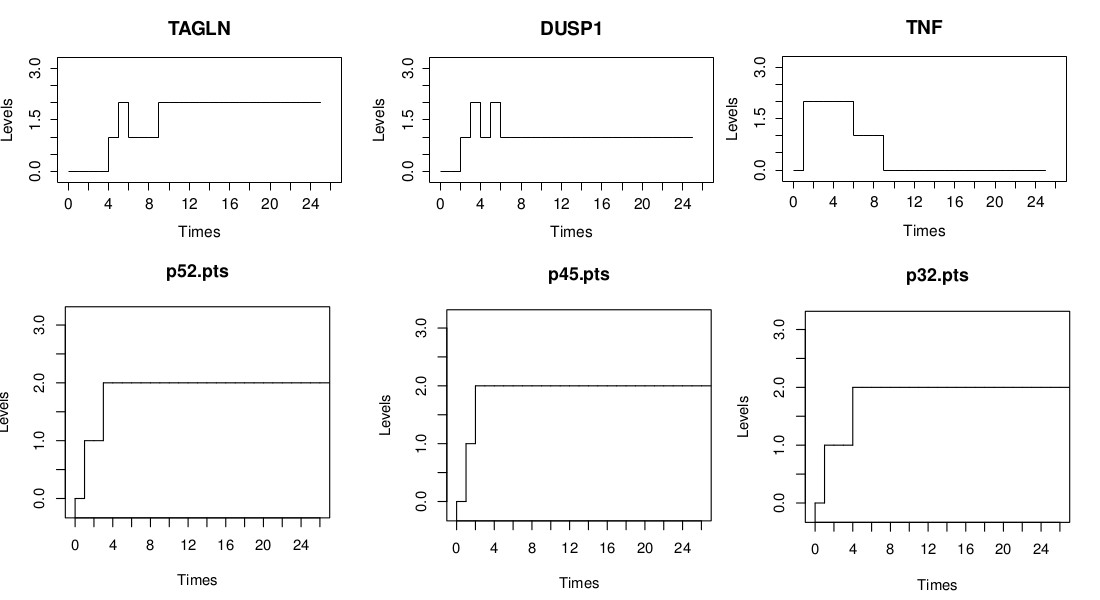
\includegraphics[scale=0.2]{figs/ph11-5-1.jpg}
\end{center}


\pause
\begin{itemize}
  \item Le temps de propagation du signal dans le réseau.
  \item différentiation du temps des activations et des inibitions
  \item Les simulations pour $r_{a}=10.0  \neq r_{i}=0.2$ et $sa = 50 $
\end{itemize}

\textcolor{couleurtheme}{$\Rightarrow$} \fbox{\tval{\large Analyse???}} \textcolor{couleurtheme}{$\Leftarrow$}

\end{frame}

\begin{frame}[c]
  \frametitle{Avancement sur la qualité du réseau en PH et de la compréhension des paramètres}
  
 \begin{center}
  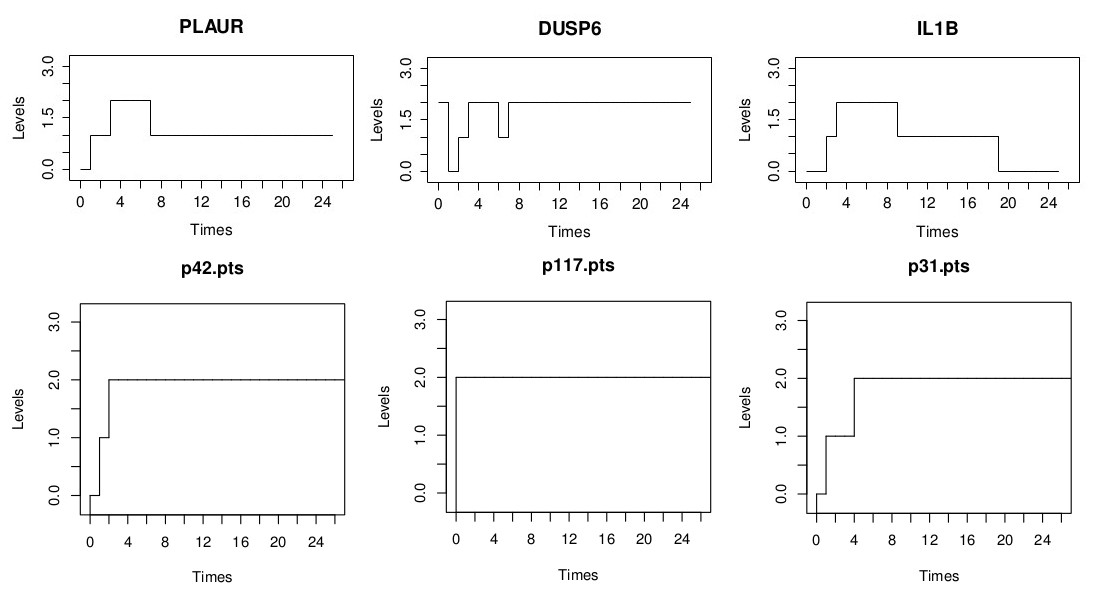
\includegraphics[scale=0.2]{figs/ph11-5-2.jpg}
\end{center}


\pause
\begin{itemize}
  \item Le temps de propagation du signal dans le réseau.
  \item différentiation du temps des activations et des inibitions
  \item Les simulations pour $r_{a}=10.0  \neq r_{i}=0.2$ et $sa = 50 $
\end{itemize}

\textcolor{couleurtheme}{$\Rightarrow$} \fbox{\tval{\large Analyse???}} \textcolor{couleurtheme}{$\Leftarrow$}

\end{frame}

\begin{frame}[c]
  \frametitle{Avancement sur la qualité du réseau en PH et de la compréhension des paramètres}
  
 \begin{center}
  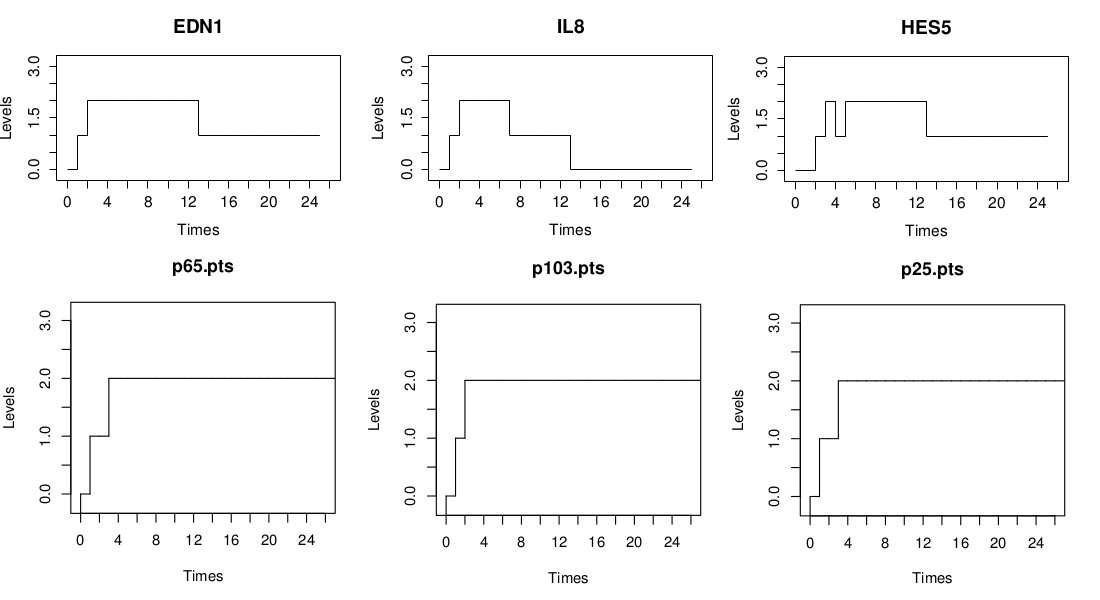
\includegraphics[scale=0.2]{figs/ph11-5-3.jpg}
\end{center}


\pause
\begin{itemize}
  \item Le temps de propagation du signal dans le réseau.
  \item différentiation du temps des activations et des inibitions
  \item Les simulations pour $r_{a}=10.0  \neq r_{i}=0.2$ et $sa = 50 $
\end{itemize}

\textcolor{couleurtheme}{$\Rightarrow$} \fbox{\tval{\large Analyse???}} \textcolor{couleurtheme}{$\Leftarrow$}

\end{frame}

\begin{frame}[c]
  \frametitle{Avancement sur la qualité du réseau en PH et de la compréhension des paramètres}
  
 \begin{center}
  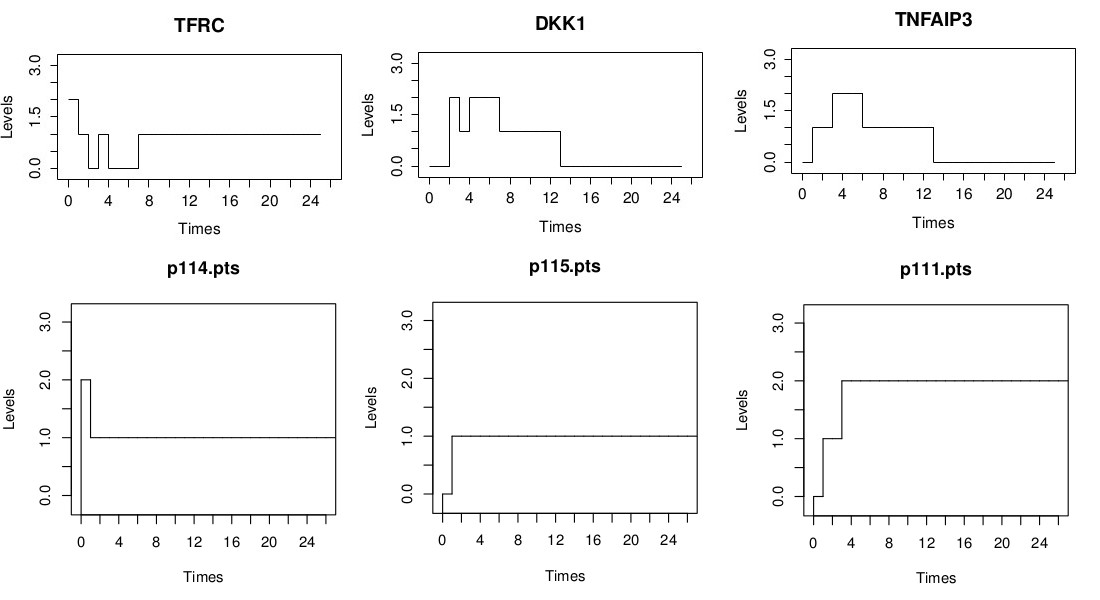
\includegraphics[scale=0.2]{figs/ph11-5-4.jpg}
\end{center}


\pause
\begin{itemize}
  \item Le temps de propagation du signal dans le réseau.
  \item différentiation du temps des activations et des inibitions
  \item Les simulations pour $r_{a}=10.0  \neq r_{i}=0.2$ et $sa = 50 $
\end{itemize}

\textcolor{couleurtheme}{$\Rightarrow$} \fbox{\tval{\large Analyse???}} \textcolor{couleurtheme}{$\Leftarrow$}

\end{frame}

% autre avancements

\begin{frame}[c]
  \frametitle{Avancement sur la qualité du réseau en PH et de la compréhension des paramètres}
  
 \begin{center}
  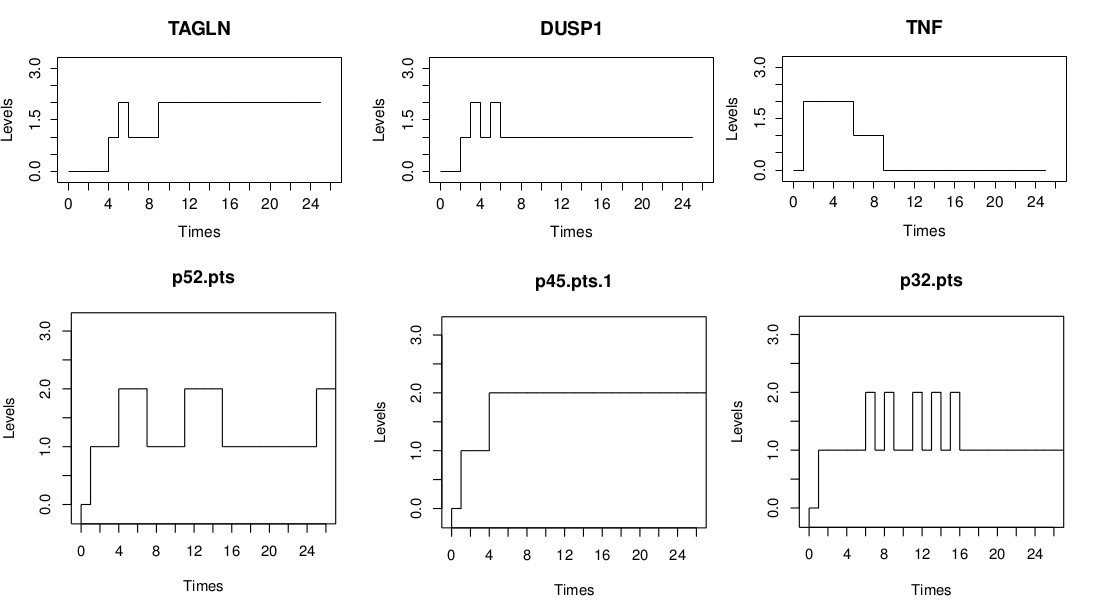
\includegraphics[scale=0.2]{figs/ph12-3-1.jpg}
\end{center}


\pause
\begin{itemize}
  \item Modification manuelle du réseau
  \item modification des prédécésseurs directes.
  \item Les simulations pour $r_{a} = r_{i}=10.0$ et $sa = 50 $
\end{itemize}

\textcolor{couleurtheme}{$\Rightarrow$} \fbox{\tval{\large Analyse???}} \textcolor{couleurtheme}{$\Leftarrow$}

\end{frame}


\begin{frame}[c]
  \frametitle{Avancement sur la qualité du réseau en PH et de la compréhension des paramètres}
  
 \begin{center}
  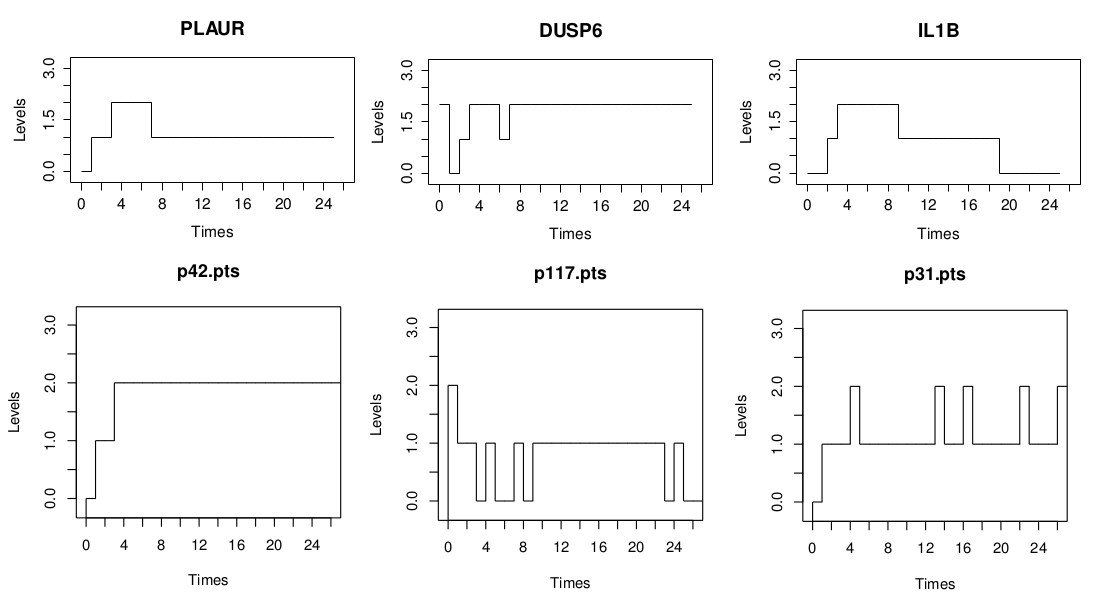
\includegraphics[scale=0.2]{figs/ph12-3-2.jpg}
\end{center}


\pause
\begin{itemize}
  \item Modification manuelle du réseau
  \item modification des prédécésseurs directes.
  \item Les simulations pour $r_{a} = r_{i}=10.0$ et $sa = 50 $
\end{itemize}

\textcolor{couleurtheme}{$\Rightarrow$} \fbox{\tval{\large Analyse???}} \textcolor{couleurtheme}{$\Leftarrow$}

\end{frame}

\begin{frame}[c]
  \frametitle{Avancement sur la qualité du réseau en PH et de la compréhension des paramètres}
  
 \begin{center}
  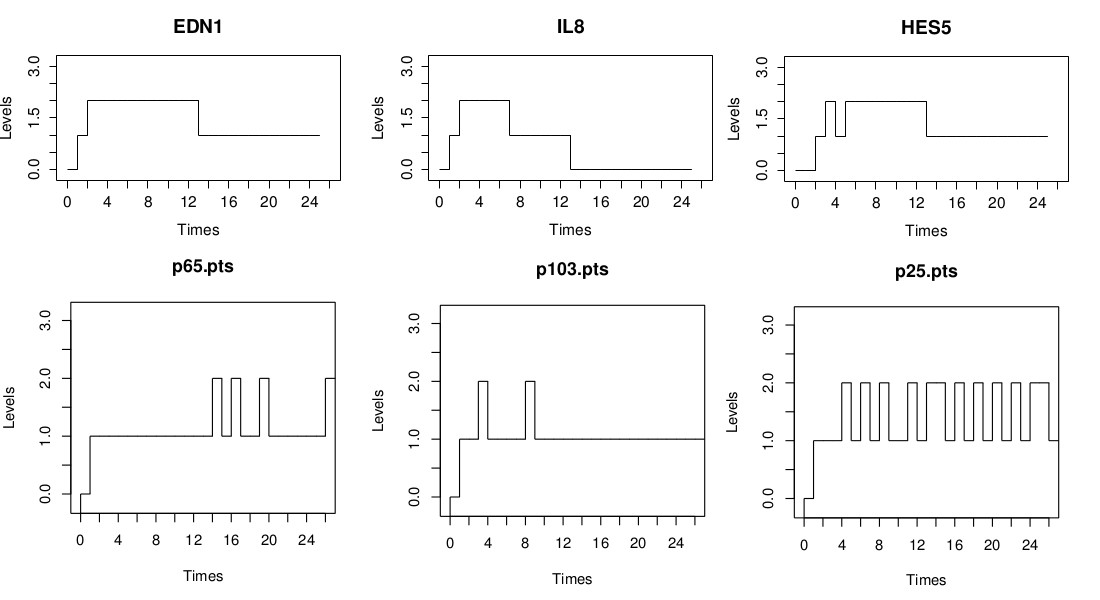
\includegraphics[scale=0.2]{figs/ph12-3-3.jpg}
\end{center}


\pause
\begin{itemize}
  \item Modification manuelle du réseau
  \item modification des prédécésseurs directes.
  \item Les simulations pour $r_{a} = r_{i}=10.0$ et $sa = 50 $
\end{itemize}

\textcolor{couleurtheme}{$\Rightarrow$} \fbox{\tval{\large Analyse???}} \textcolor{couleurtheme}{$\Leftarrow$}

\end{frame}

\begin{frame}[c]
  \frametitle{Avancement sur la qualité du réseau en PH et de la compréhension des paramètres}
  
 \begin{center}
  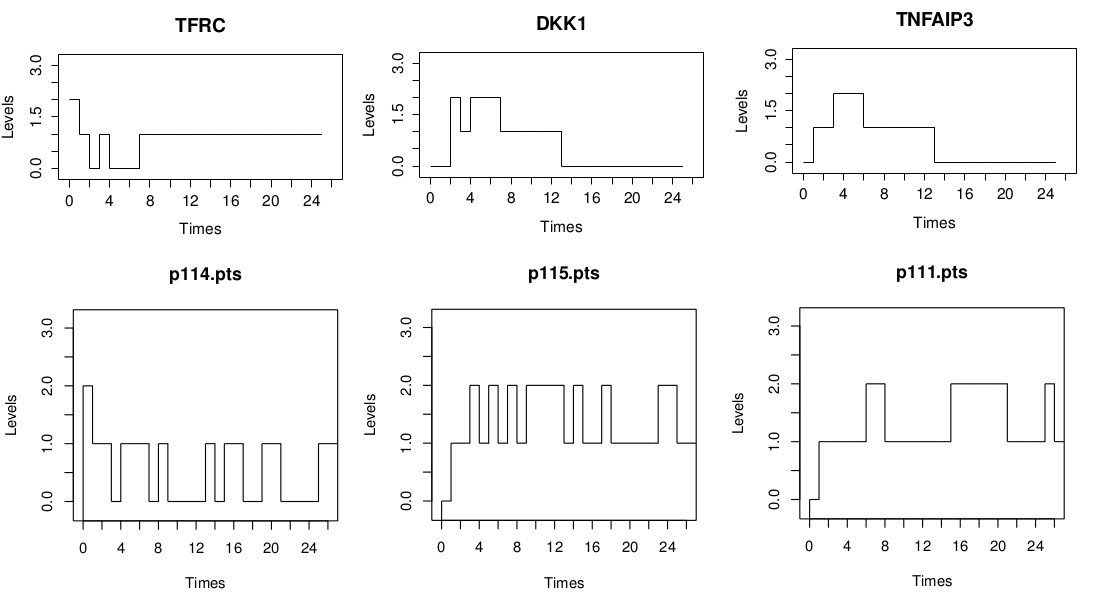
\includegraphics[scale=0.2]{figs/ph12-3-4.jpg}
\end{center}


\pause
\begin{itemize}
  \item Modification manuelle du réseau
  \item modification des prédécésseurs directes.
  \item Les simulations pour $r_{a} = r_{i}=10.0$ et $sa = 50 $
\end{itemize}

\textcolor{couleurtheme}{$\Rightarrow$} \fbox{\tval{\large Analyse???}} \textcolor{couleurtheme}{$\Leftarrow$}

\end{frame}